\chapter{Grundlagen der Plugin-Entwicklung}
\label{cha:Grundlagen}

\section{Entwicklungsumgebungen}
\label{sec:Entwicklungsumgebungen}

\subsection{Visual Studio Code}

Die erste offizielle Version von Visual Studio Code, häufig 
abgekürzt auch als VS Code, wurde im April 2016 \cite{VSCodeReleaseDate}
von Microsoft veröffentlicht. Die Idee hinter VS Code
war, einen möglichst einfachen Code Editor anzubieten, 
welcher nur die wichtigsten und besten Funktionen für EntwicklerInnen 
beinhaltet. Es hob sich somit von anderen Entwicklungsumgebungen (engl. IDEs)
wie der Visual-Studio-Reihe von Microsoft ab, da es ein sehr 
leichtgewichtiger Editor war, welcher trotzdem mit einer großen 
Menge an Programmiersprachen arbeiten konnte und für diese auch 
Microsofts automatische Codevervollständigung namens „IntelliSense“ 
unterstützte. Weiters war Visual Studio Code das erste Produkt der Visual 
Studio Familie, welches plattformübergreifen für Windows, Linux und macOS 
angeboten wurde \cite{VSCodePreview}.

Aus den Stack Overflow Developer Surveys\cite{StackOverflowSurvey,StackOverflowSurvey2023}
der vergangenen Jahre kann 
der rasche Aufstieg von VS Code beobachtet werden. Während es im 
Jahr der Veröffentlichung nur von etwa 7,2 Prozent der EntwicklerInnen 
genutzt wurde, war es zwei Jahre später bereits (wenn auch knapp) 
die meistgenutzte IDE mit 34,9 \%. In der aktuellsten Umfrage von 
2023 war es der klare Sieger und wurde vom 73,71\% der Abstimmenden 
aktiv genutzt\cite{StackOverflowSurvey,StackOverflowSurvey2023}.

Ein Grund für diesen Erfolg mag vermutlich die Möglichkeit 
zur Entwicklung und zum Anbieten von Extensions sein. Durch die direkte 
Einbindung des Visual Studio Marketplace in VS Code bildete sich über die 
Jahre eine große Community, die eine enorme Anzahl von Extensions 
entwickelt, verbessert und betreut. Durch solche, oft 
von der Community erstellte, Extensions kann VS Code auch eine 
enorme Anzahl von Programmiersprachen unterstützen.


\subsection{IntelliJ IDEA}

IntelliJ IDEA wurde erstmals im Januar 2001 \cite{IntelliJReleasePage}
von dem Unternehmen 
JetBrains veröffentlicht. Im Gegensatz zu VS Code handelt 
es sich bei IntelliJ um eine vollausgestattetes Integrate Development Environment (IDE),
welche speziell auf die Entwicklung 
von Programmen in den Programmiersprachen Java, Kotlin und Groovy ausgelegt ist. 
IntelliJ IDEA wird in einer freien, Open Source 
\enquote{Community Edition} \cite{IntelliJCommunityEditionGithub} sowie in einer kommerziellen Form 
\enquote{IntelliJ IDEA Ultimate} angeboten \cite{HagosTed2022BII:}. 

Aufgrund der Spezialisierung auf JVM-kompatible Sprachen unterstützt 
die IntelliJ Community Edition nur eine relativ kleine Auswahl an 
Sprachen, Frameworks und Build Tools. Während IntelliJ IDEA Ultimate 
den Umfang an Features schon deutlich erweitert, bietet JetBrains auch 
noch weitere kommerzielle IDEs an. Diese sind alle für unterschiedliche 
Programmiersprachen oder Sprachfamilien ausgelegt. Einige der bekanntesten 
sind dabei CLion für die Sprachen C und C++, Rider für die .NET Sprachen, 
PhpStorm für PHP und WebStorm für JavaScript. Zum aktuellen 
Zeitpunkt sind es insgesamt elf verschiedene IDEs, die von JetBrains 
angeboten werden und die alle auf der IntelliJ Platform basieren. Das 
bedeutet nicht nur, dass sich all diese IDEs in der Verwendung und im 
Aussehen sehr ähnlich sind, sondern auch, dass ein Plugin, welches für 
die allgemeine IntelliJ Platform entworfen wurde, 
auch für mehrere IDEs dieser Plattform veröffentlicht werden kann \cite{IntelliJSDKDocumentation}.

Im Gegensatz zu Visual Studio Code ist IntelliJ ein schwergewichtiger
Editor, der sehr viel Funktionalität schon von Grund auf eingebaut 
hat. Die EntwicklerInnen sind hier nicht so stark auf Plugins angewiesen.
Dies lässt sich auch durch die Anzahl von Plugins erkennen, die auf dem 
JetBrains Marketplace angeboten werden. Für die IntelliJ Platform gibt 
es aktuell etwas über 7.500 Plugins, die in die IDE integriert werden können 
\cite{IntelliJMarketplace}.
Für Visual Studio Code sind es hingegen inzwischen über 51.000 Extensions
\cite{VSCodeMarketplace}.


\section{Programmiersprachen}
\label{sec:Programmiersprachen}

\subsection{TypeScript}

Die Programmiersprache TypeScript wurde erstmalig am 1. Oktober 2012 
\cite{TypeScriptCodePlexArchived} von 
Microsoft in Form eines Open-Source-Projekts veröffentlicht. Entworfen wurde sie 
von Anders Hejlsberg, der zuvor auch die Programmiersprache C\# entworfen hatte. 

Die grundsätzliche Idee der Sprache ist, eine typsichere, kompilierte, und somit 
bessere Version von JavaScript zu sein. JavaScript ist aufgrund des Erfolgszugs
des World Wide Web zu einer sehr wichtigen Sprache geworden und war auch schon 2012 
aus den TOP-Listen für Programmiersprachen nicht mehr wegzudenken 
\cite{StackOverflowSurvey,TIOBEIndex,PYPL}. 
Webseiten setzen heute sehr stark auf JavaScript, um durch interaktive Elemente 
die User Experience zu verbessern oder um neue Funktionalität anbieten zu können. 
Durch Node.js kann JavaScript nicht nur im Browser 
verwendet werden, sondern es können auch Desktop-, Server- oder mobile-Anwendungen 
in JavaScript entwickelt werden \cite{rozentals2017mastering}.
Durch diesen großen Umfang an Möglichkeiten, die 
JavaScript dadurch bietet, werden auch immer größere Projekte damit entwickelt. 
Und hier kommen die großen Schwächen von JavaScript zu tragen. 
Je größer die Projekte werden und je mehr EntwicklerInnen an einem Projekt 
mitarbeiten, desto mehr Fehler entstehen aufgrund der fehlenden Typsicherheit
und der fehlenden statischen Überprüfungen (wie zum Beispiel bei einem Compiler). 
Beide Schwachstellen versucht TypeScript auszubessern.

TypeScript Quellcode wird mithilfe des TypeScript Compilers \emph{tsc} in JavaScript 
Dateien transpiliert. Dadurch kann auf die Popularität und Verbreitung von JavaScript 
aufgebaut werden. TypeScript ist überall dort verwendbar, wo JavaScript 
ausführbar ist. Weiters ist TypeScript eine echte Übermenge von JavaScript. 
Es gilt also: „Any valid .js file can be renamed .ts and be compiled with other 
TypeScript file.” \cite{MaharryDanTR}. 

Jedoch bietet TypeScript eine Menge von Vorteilen 
gegenüber Javascript.
\begin{itemize}
  \item Durch den Kompilierschritt mit dem tsc Compiler wird der 
    Code vor der Ausführung automatisch auf Validität geprüft. 
    Es entfällt also die Notwendigkeit für einen zusätzliches Werkzeug 
    zur statischen Programmanalyse, wie JSLint. 
    Dieser Kompilierschritt kann natürlich auch in eine 
    CI/CD Pipeline eingebunden werden, um auch bei Änderungen in einem
    Repository Informationen über die Gültigkeit des Quellcodes zu erhalten.
  \item Durch die statische Typisierung können Programmierfehler bezüglich
    der Verwendung von Variablen vermieden werden. Auch die Unterstützung 
    durch verschiedene IDEs, zum Beispiel mittels IntelliSense kann durch 
    Typen verbessert werden. Dies ist nicht nur bei der Zusammenarbeit hilfreich, 
    sondern kann auch die Arbeit jeder einzelnen EntwicklerIn beschleunigen.
  \item In TypeScript können Klassen erstellt werden, deren Eigenschaften mit 
    Zugriffsmodifikatoren (\emph{private}/\emph{public}) versehen sind.
  \item TypeScript unterstützt Vererbung, Schnittstellen und generische Programmierung.
  \item In TypeScript können bereits bestehende JavaScript-Bibliotheken 
    verwendet werden. Weiters ist es möglich, durch zusätzliche Dateien 
    Typinformationen zu \linebreak
    JavaScript-Bibliotheken zu liefern.
\end{itemize}

\subsection{Java}

Die Entwicklung der Programmiersprache Java begann im Jahr 1991. Java 
wurde von James Gosling, Mike Sheridan und Patrick Naughton entworfen \cite{WinnieDoug2021EJfA}.
Java wurde erstmals im Jahr 1995 von Sun Microsystems veröffentlicht. 
Im Januar 2010 wurde Sun Microsystems von der Oracle Corporation übernommen, 
welche seitdem auch Java weiterentwickelt.

Das Design und vor allem die Syntax der Sprache war stark von C und C++ inspiriert \cite{ArnoldKen1996TJpl}, 
um EntwicklerInnen einen leichten Umstieg auf die neue Sprache Java zu ermöglichen. 
Allerdings versuchte Java die teils sehr komplexen (wenn auch effektiven) 
Sprachfeatures von C++ etwas zu vereinfachen. Java sollte eine einfach, objektorientierte 
und robuste Sprache werden. Die Funktionalität die Java zu dem großen Erfolg verhalf, 
den sie später hatte, war das Prinzip
\begin{quote}\begin{english}\enquote{write once, run anywhere}\end{english}\end{quote}
(WORA) \cite{SharanKishori2022BJ1f}. 

Im Gegensatz 
zu den zuvor gängigen Programmiersprachen muss Java nämlich nicht für bestimmte 
Hardwarearchitekturen kompiliert werden. Java-Programme werden in eine 
Zwischensprache, den sogenannten Java Bytecode, kompiliert. Dieser Bytecode
kann dann von einer Java Virtual Machine (JVM) ausgeführt werden. Diese JVM ist
im Grunde ein eigenständiges Programm, welches mit der Java Runtime Environment 
(JRE) mitgeliefert wird. Ein kompiliertes Java-Programm kann also auf 
allen Geräten ausgeführt werden, auf denen eine passende JRE installiert ist. 
So ist es zum Beispiel auch möglich, Java für die Entwicklung von Android nativen
Apps auf Mobilgeräten zu benutzen.

Ein weiterer Vorteil gegenüber älteren Sprachen wie C++ ist die
automatisierte Speicherverwaltung. Diese funktioniert mithilfe eines 
sogenannten \enquote{Garbage Collectors} welcher nicht mehr benötigten Speicher
am Heap bereinigt und freigibt. Man kann also beliebig neue Objekte im Speicher
allokieren und muss sich nicht um die Deallokierung der zuvor erstellten Objekte
kümmern. Auf diese Weise können häufige Programmierfehler wie Memory Leaks unterbunden werden.

Java unterstützt sowohl das objektorientierte, das prozedurale als auch das funktionale 
Programmierparadigma. Der Fokus liegt allerdings stark auf der Objektorientierung. 
Dazu bietet Java Möglichkeiten zur Abstraktion durch Verwendung von Klassen, Information Hiding
mithilfe von Zugriffsmodifikatoren (\emph{public}/\emph{private}/\emph{protected}/\linebreak
\emph{package}), Vererbung, 
Schnittstellen, Polymorphismus, Überladen von Methoden, generischer Programmierung, 
Ausnahmebehandlung und vieles mehr.

% //TODO OPTIONAL section: LSP

\section{Aufbau der Plugin API}
\label{sec:AufbauDerPluginAPI}

Um die Bezeichnungen für IntelliJ Plugins und VS Code Extensions zu vereinheitlichen,
wird in den folgenden Abschnitten und Kapiteln \emph{Plugin} als Überbegriff
verwendet, der auch VS Code Extensions einschließt.

\subsection{Visual Studio Code}

Visual Studio Code bietet für Plugins zwei Arten der
Interaktion, welche zusammenspielen, um Plugins zu ermöglichen. 
Das Extension Manifest und die eigentliche API.
\subsubsection{Extension Manifest} 
  Das Extension Manifest befindet sich in der Datei \emph{package.json}.
  In dieser werden statische Einstellungen vorgenommen und
  Metainformationen über das Plugin bekannt gegeben. So kann hier unter
  anderem Name, Beschreibung, Herausgeber und Lizenzvereinbarungen
  eingestellt werden. Weiters definiert das Manifest eine sogenannte
  JavaScript- oder TypeScript-Datei \emph{main}  und dazu passende
  \emph{Activation Events} und \emph{Contribution Points}
  \cite{VSCodeExtensionAPIExtensionManifest,VSCodeExtensionAPIExtensionAnatomy}.
  \begin{description}
    \item[Activation Events] bestimmen den Zeitpunkt, an dem das Plugin zum ersten Mal
      aktiviert wird. Dabei wird die \emph{activate} Funktion der zuvor definierten
      \emph{main}-Datei ausgeführt. Der Aktivierungszeitpunkt sollte immer so spät wie
      möglich gewählt werden, um VS Code möglichst wenig zu verlangsamen und
      das Plugin erst bei Bedarf (on demand) zu Laden. Allerdings
      muss die Aktivierung erfolgen bevor die erste Funktionalität des
      Plugins erwartet wird. Typische Aktivierungsereignisse sind \emph{onCommand}
      , \emph{onDebug}, \emph{onView} oder \emph{onStartupFinished}.
      Wurde das Plugin einmal aktiv, bleibt es auch aktiv bis VS Code wieder geschlossen
      wird oder das Plugin entfernt oder deaktiviert wird. Hierfür gibt es optional
      noch eine \emph{deactivate}-Funktion in der \emph{main}-Datei, welche für etwaige
      Aufräumarbeiten genutzt werden kann
      \cite{VSCodeExtensionAPIActivationEvents,VSCodeExtensionAPIExtensionAnatomy}.
    \item[Contribution Points] legen fest, welche Funktionalität das Plugin anbietet
      und somit auch, welche zusätzlichen UI-Elemente
      dem Nutzer in VS Code angezeigt werden sollen.
      Hier ist es beispielsweise möglich, Visual Studio Code mit neuen Befehlen (\enquote{Commands}),
      Menüs und Submenüs, Views für das Anzeigen von Plugin-definiertem Content,
      Keyboard Shortcuts, Unterstützung für neue Sprache und vieles mehr auszustatten 
      \cite{VSCodeExtensionAPIContributionPoints}.
  \end{description}
\subsubsection{Visual Studio Code API} 
  Die eigentliche VS Code API kann in jeder TypeScript-Datei 
  (zum Beispiel auch in der Datei \emph{main}) genutzt werden. 
  Hierfür wird das Modul \emph{vscode} importiert. 
  Dieses beinhaltet eine vollständige Definition der angebotenen
  Schnittstelle, auf welche zugegriffen werden kann 
  \cite{VSCodeExtensionAPIExtensionAnatomy,VSCodeExtensionAPIVSCodeAPI}.
\begin{JsCode}
    import * as vscode from 'vscode';

    export function activate(context: vscode.ExtensionContext) {
      vscode.window.showInformationMessage('Hello World!');
    } 
\end{JsCode}
  Über diese API kann zum Beispiel festgelegt werden, durch welchen Code
  die zuvor definierten Contribution Points implementiert werden sollen.
  Der Plugin Code wird in VS Code nicht im selben Prozess wie das
  Hauptprogramm ausgeführt, sondern abgekapselt in einem seperaten 
  \enquote{extension host process}. Dadurch kann verhindert werden, dass
  Plugins die Performance und die Interaktivität von VS Code negativ beinflussen 
  \cite{VSCodeArchitecture,VSCodeApproachToExtensibility}.
\subsubsection{Ablauf}
  Wie in Abbildung \ref{fig:diagram_VSCodeExtensionArchitecture} zu sehen ist,
  analysiert VS Code zuerst das Extension Manifest des Plugins.
  Je nachdem welche Activation Points definiert sind, wird zu einem
  bestimmten Zeipunkt die \emph{activate}-Funktion aufgerufen. In dieser 
  können dann mithilfe der API Event Handler registriert werden. 
  Die registrierten Handler werden dann während der Ausführung und Verwendung
  von VS Code aufgerufen und können so beliebigen Code ausführen.
  \begin{figure}
    \centering
    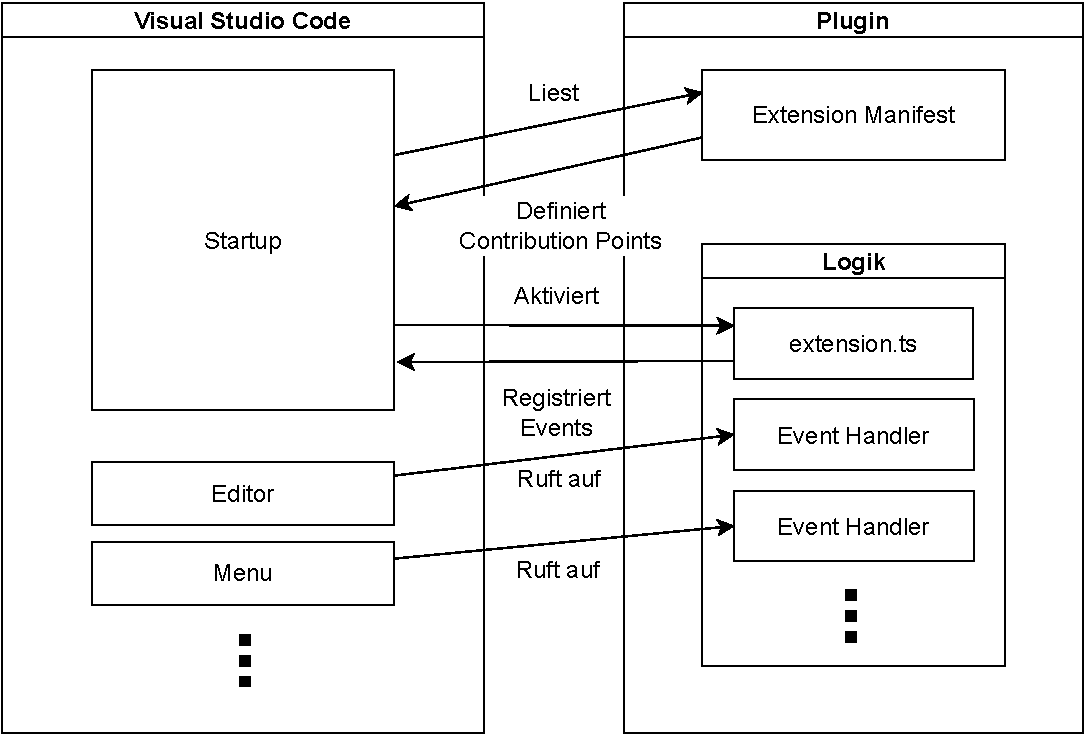
\includegraphics[width=.95\textwidth]{diagram_VSCodeExtensionArchitecture}
    \caption{Übersicht über den Ablauf eines VS Code Plugins.}
    \label{fig:diagram_VSCodeExtensionArchitecture}
  \end{figure}   

\subsection{IntelliJ IDEA}

Der Aufbau der Plugin-Architektur wirkt bei IntelliJ im ersten Moment 
gleich wie bei VS Code. Es gibt auch hier ein \emph{Plugin Configuration File}, 
sowie ein Modul mit API Schnittstellen \cite{IntelliJPlatformSDKPluginStructure}.
Der große Unterschied liegt allerdings in der Funktionsweise und der Interaktion
mit den Plugins sowie der Art, wie der auszuführende Code angegeben wird.
\subsubsection{Plugin Configuration File}
  Die Konfiguration eines Plugins liegt in der Datei \emph{plugin.xml} und
  beinhaltet, äquivalent zum Extension Manifest in VS Code, alle für das Plugin
  notwendigen Meta-Informationen. So können auch hier Werte wie der Name,
  eine Beschreibung und die aktuelle Versionsnummer angegeben werden.
  Für die Funktionen, die das Plugin mitbringt, gibt es Actions, Extension Points
  und Listener. Hier ist anzumerken, dass es sich sowohl bei den Extension Points
  als auch den Listenern immer um eine Zuordnung eines Interfaces
  (meist definiert von IntelliJ) zu einer Implementierung (definiert durch das Plugin)
  handelt. Weiters ist es nicht nötig einen speziellen Aktivierungszeitpunkt
  festzulegen, da dieser durch die Zuordnung der auszuführenden Klassen sowieso durch 
  die Konfigurationsdatei festgelegt wird \cite{IntelliJPlatformSDKPluginConfigurationFile}. 
  Eine Besonderheit an IntelliJ ist,
  dass Plugins auch eigene Extension Points definieren können, um weiteren Plugins
  das Erweitern des ursprünglichen Plugins zu ermöglichen
  \cite{IntelliJPlatformSDKExtensionPoints}.
\subsubsection{IntelliJ Platform SDK}
  Die API für IntelliJ Plugins ist in mehreren Paketen des IntelliJ 
  Platform SDK enthalten. Diese API enthält auch die unterschiedlichen
  Interfaces, welche dann in Form von Extension Points oder Listenern implementiert
  werden können. Die Implementierung eines Plugins kann in den Sprachen Java
  und Kotlin erledigt werden. Da die Plugin API allerdings auf Java basiert, können
  nicht alle Sprachfeatures von Kotlin problemlos genutzt werden 
  \cite{IntelliJPlatformSDKConfiguringKotlinSupport}.
\subsubsection{Ablauf}
  Wie in Abbildung \ref{fig:diagram_IntelliJExtensionArchitecture} zu sehen ist,
  analysiert IntelliJ zuerst das Plugin Configuration File.
  Je nachdem, welche Funktionalität vom Plugin angeboten wird, werden
  von IntelliJ automatisch die entsprechenden Event Handler 
  auf die unterschiedlichen Extension Points registriert. 
  Die registrierten Handler werden dann während der Ausführung und Verwendung
  von IntelliJ aufgerufen und können so beliebigen Code ausführen.
  \begin{figure}
    \centering
    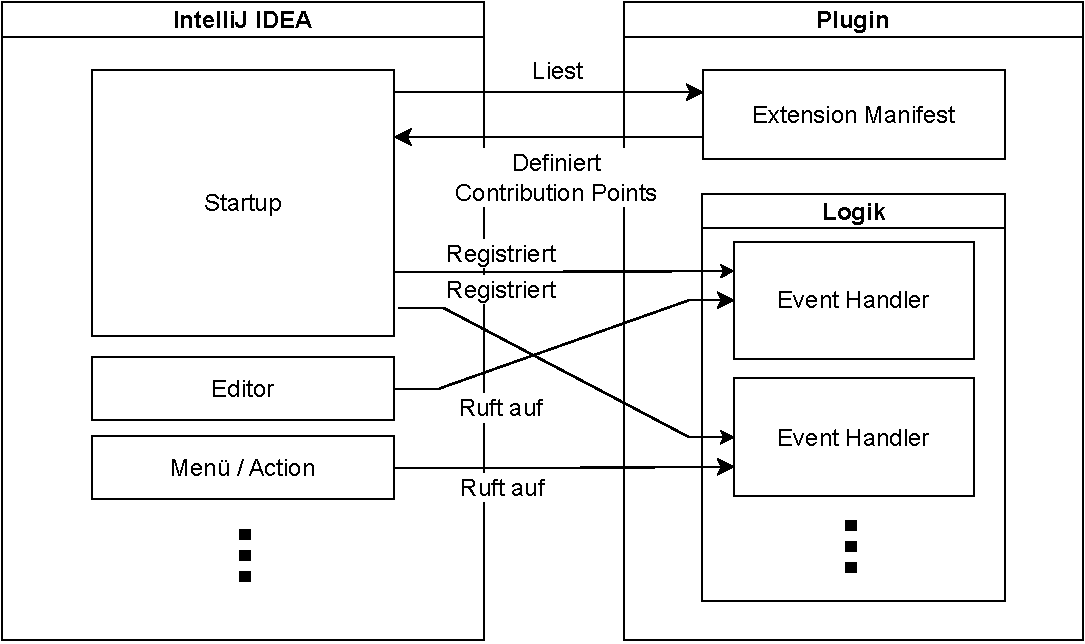
\includegraphics[width=.95\textwidth]{diagram_IntelliJExtensionArchitecture}
    \caption{Übersicht über den Ablauf eines IntelliJ Plugins.}
    \label{fig:diagram_IntelliJExtensionArchitecture}
  \end{figure}   

\section{Funktionalität der Plugin API}
\label{sec:FunktionalitätDerPluginAPI}

\subsection{Visual Studio Code}

Die VS Code API erlaubt es, VS Code durch Commands, Code Completion und Spracherweiterung, 
Themes, Custom Editor, Notebooks, Views, Source Control, Debugger, Tests und vielem mehr zu
erweitern. Um dies zu ermöglichen, werden unter anderem auch Einstellungen, Datenspeicherung
und verschiedene Arten der Ein- und Ausgabe von Daten bereitgestellt. In den folgenden Abschnitten
werden die wichtigsten Elemente genauer vorgestellt.

\subsubsection{Commands und Menüs}
  Commands ermöglichen es dem Plugin, bestimmten Code sozusagen \enquote{auf Befehl} auszuführen.
  So können häufig wiederkehrende Aufgaben der BenutzerInnen ganz einfach automatisiert werden.
  Um einen Command anzulegen, muss dieser im Extension Manifest definiert werden. Dabei muss
  das Plugin mindestens eine eindeutige Bezeichnung und zur Darstellung verwendeten Titel angeben.
  Optional können auch eine Kategorie, ein Icon und eine Kurzbezeichnung bestimmt werden. 
  Weiters ist es möglich eine Bedingung festzulegen, die beeinflusst, wann
  der Command verwendbar ist und wann nicht \cite{VSCodeExtensionAPIContributionPointsCommands}.
\begin{JsCode}
    "commands": [
      {
        "command": "vscodeplugindemo.helloWorld",
        "title": "Hello World",
      }
    ] 
\end{JsCode}

  Welcher Code dann ausgeführt wird, muss über die API festgelegt werden. So wird meist
  in der \emph{activate}-Funktion mithilfe von \emph{registerCommand} oder \emph{registerTextEditorCommand}
  ein Callback festgelegt, welches aufgerufen werden soll. Wichtig ist hier, dass
  die register-Funktionen ein Objekt retournieren, welches \emph{Disposable} implementiert.
  Dieses muss der API bekannt gegeben werden. 
  Die API kümmert sich dann auch um das Deaktivieren des Commands, falls zum Beispiel
  die Erweiterung deaktiviert werden sollte \cite{VSCodeExtensionAPICommands}.
\begin{JsCode}
    context.subscriptions.push(vscode.commands.registerCommand('vscodeplugindemo.helloWorld', () => {
      vscode.window.showInformationMessage('Hello World from VsCodePluginDemo!');
    })); 
\end{JsCode}

  Um einen Command aufzurufen können die Nutzer direkt nach dem Command suchen (Tastenkombination Strg+Shift+P).
  Komfortabler ist es allerdings, den Nutzern direkt einen passenden Menüeintrag oder ein Keybinding
  bereitzustellen. Menüeinträge können dabei an verschiedenen Stellen in der
  Benutzeroberfläche eingehängt werden.
  Gängig sind hierfür die Titelleiste des Editors, verschiedene Kontext-Menüs, der Dialog
  zum Anlegen einer neuen Datei, die Titelleiste einer bestimmten View oder ein neues Submenü in der Menüleiste.
  Sowohl Menüs als auch Keybindings können im Manifest registriert werden
  \cite{VSCodeExtensionAPIContributionPointsMenus}.
  % // TODO OPTIONAL paragraph: about calling commands from code
\subsubsection{Spracherweiterungen}
  Ein wichtiger Teil der VS Code Plugin API sind Language Extensions. Visual Studio Code unterscheidet
  bei diesen Funktionen zwischen Highlighting, Language Features und Snippets.
  \begin{description}
    \item[Highlighting] 
      Das Syntax Highlighting wird in VS Code durch eine TextMate-\linebreak
      Grammatik erledigt \cite{TextMateGrammar}.
      Diese Grammatik wird dabei nicht nur für das Highlighting genutzt, sondern sie ist auch für das \enquote{Tokenization}
      zuständig. Durch eine Codeanalyse anhand der gegebenen Grammatik wird der Text in kleine 
      zusammengehörige Abschnitte (sogenannte Tokens) unterteilt. Diese Tokens werden zusätzlich noch 
      klassifiziert, sodass zum Beispiel zwischen Kommentaren, Zeichenkettenliteralen, regulären Ausdrücken und Code unterschieden werden kann.
      Die Grammatik wird hierfür in einer einfachen Json-Datei im Plugin Projektordner abgelegt und dann per Manifest
      unter dem Contribution Point \emph{grammar} eingebunden. Mithilfe solcher Grammatiken können auch bereits bestehende
      Grammatiken erweitert werden. Bei der Auswahl von Scopes, die durch die Grammatik definiert werden, sollte man sich
      an die Namenskonventionen von TextMate halten. Scopes mit diesem Namensschema werden auch von vielen Themes unterstützt werden
      \cite{VSCodeExtensionAPISyntaxHighlightGuide}.
      Um die Kategorisierung von bestimmten Tokens noch genauer zu erledigen, gibt es in VS Code auch \enquote{Semantic Highlighting}. 
      Es kann in der API ein \emph{DocumentSemanticTokensProvider} registriert werden,
      welcher den Code analysiert und zusätzliche (zum Beispiel kontextabhängige) Informationen über die Tokens bereitstellt
      \cite{VSCodeExtensionAPISemanticHighlightGuide}.
    \item[Language Features] 
      Auch hier gibt es statisch definierte und programmatische Language Features.
      Statisch kann unter dem Contribution Point \emph{languages} eine Reihe von Informationen angegeben werden,
      die es VS Code erlauben, die User Experience stark zu verbessern. So kann man unter anderem festlegen,
      mit welchen Zeichen Kommentare eingeleitet werden, oder welche Klammern es gibt, damit VS Code das Zuklappen erlauben kann.
      Zusammengehörige Paare von Zeichen (also Klammern, Anführungszeichen, u.s.w.) können automatisch geschlossen werden.
      Und sogar für das automatische Einrücken der nächsten Zeile bei einem Zeilenumbruch kann eine Regel erstellt werden
      \cite{VSCodeExtensionAPILanguageConfigurationGuide}.
      Programmatisch ist das Erweitern von Language Features etwas komplexer, allerdings steigt auch die
      Menge an Möglichkeiten. In der API können verschiedene Provider registriert werden, durch die Features wie
      \enquote{Go to Definition}, \enquote{IntelliSense} Codevervollständigung oder diagnostische Fehleranalysen und
      entsprechende Verbesserungsvorschläge ermöglicht werden
      \cite{VSCodeExtensionAPIProgrammaticLanguageFeatures}. 
      Grundsätzlich ist es auch möglich, für einzelne
      Features einen Provider zu registrieren. Allerdings empfiehlt es sich, bei der Einbindung einer neuen
      Sprache, einen \enquote{Language Server} und das Language Server Protocol zu nutzen. Diese Lösung
      bringt nicht nur Performanceverbesserungen im Editor sondern der Language Server kann auch für 
      andere Editoren wiederverwendet werden, ohne dass er mehrfach implementiert werden muss. \cite{GunasingheNadeeshaan2022Lspa}.
      % //TODO OPTIONAL paragraph: results of existing lsp can probably be gotten by calling built-in commands. need some further research for this...
    \item[Snippets] 
      Snippets sind eine sehr einfache Form der Spracherweiterung. Es wird unter dem Contribution Point
      \emph{snippets} einfach eine Datei mit den Vorlagen angegeben. Eine Vorlage enthält dabei immer
      ein Kürzel für welches das Snippet vorgeschlagen werden soll, den zu ersetzenden Text und optional
      eine Beschreibung. Dabei können im Text auch Platzhalter genutzt werden an die der Cursor beim Einsetzen
      des Snippets springt
      \cite{VSCodeExtensionAPISnippetGuide}.
  \end{description}
\subsubsection{Benutzereingaben}
\label{sec:FunktionalitätDerPluginAPI_Benutzereingaben}
  Für die Eingabe von Daten bietet VS Code die Quick Pick API, die File Picker API
  und den Configuration Contribution Point \cite{VSCodeExtensionAPICommonCapabilities}.
  \begin{description}
    \item[Quick Pick API] gibt dem Plugin eine Möglichkeit, den Nutzern ein einfaches Eingabefenster
      anzuzeigen. Dabei kann ein Fenster mit bereits vorgegebenen Auswahlmöglichkeiten durch
      den Aufruf von \emph{showQuickPick} oder \emph{createQuickPick} erstellt werden.
      Alternativ kann man mit den Funktionen \emph{showInputBox} oder \emph{createInputBox}
      die Nutzer auch selber einen Text eingeben lassen. Die show-Funktionen bieten dabei immer
      eine einfache vorgefertigte Implementierung an. Falls diese Option nicht ausreichend ist,
      kann mit den create-Funktionen auch eine komplexere Implementierung angegeben werden.
      Weiters kann auch eine Validierung des Inputs vorgenommen werden \cite{VSCodeExtensionAPIQuickPick}.
      Möchte man mehrere solcher Dialoge als Abfolge hintereinander anzeigen, so muss dies
      selber programmiert werden. Hierfür gibt es ein Beispiel namens \emph{quickinput-sample}
      \cite{VSCodeExtensionAPIQuickInputSample}
      im Repository \emph{vscode-extension-sample} \cite{VSCodeExtensionSamples}. 
    \item[File Picker API] erlaubt das Auswählen von Ordnern oder Dateien aus dem Dateisystem
      des Betriebssystems mit der Funktion \emph{showOpenDialog}. Dabei können Optionen angegeben
      werden, die zum Beispiel beeinflussen, ob Ordner und/oder Dateien gewählt werden dürfen, 
      ob mehrere Elemente selektiert werden dürfen oder ob nach Dateinamen gefiltert werden soll
      \cite{VSCodeExtensionAPIFilePicker}.
    \item[Configuration Contribution Point] ermöglichen das Festlegen von Einstellungen,
      die von den Nutzern eingegeben und vom Plugin ausgelesen werden können. Hier können
      Einstellungen vom Typ \emph{number}, \emph{string} und \emph{boolean} definiert werden, welche dann direkt
      im User Interface der VS Code Einstellungen bearbeitet werden können.
      Einfache \emph{object}- und \emph{array}-Eigenschaften können auch im UI dargestellt werden,
      allerdings dürfen diese keine verschachtelten Objekte oder Arrays enthalten.
      Ansonsten wird in den Einstellungen nur auf die manuell zu bearbeitende
      Datei \enquote{settings.json} verwiesen.
      Für die Validierung der Einstellungen können Validierungsproperties
      von JSON Schema verwendet werden. Es ist also zum Beispiel möglich,
      ein maximum/minimum, einen regulären Ausdruck oder ein enum Array
      mit erlaubten Werten anzugeben.
      Zusätzlich ist es zu jeder Einstellung möglich, einen Titel und eine Beschreibung
      anzugeben, wobei es sogar Beschreibungen gibt, welche Markdown-Formattierungen
      enthalten dürfen \cite{VSCodeExtensionAPIContributionPointsConfiguration}.
  \end{description}
\subsubsection{Ausgaben und Anzeigen}
  Um den BenutzerInnen auch Feedback über die Ausführung des Plugin-Codes zu geben, 
  ist in VS Code für drei allgemeine Anwendungsfälle vorgesorgt 
  \cite{VSCodeExtensionAPICommonCapabilities}. 
  
  Um den BenutzerInnen eine kurze 
  Rückmeldung zu geben, können am besten Notifications genutzt werden. Diese zeigen eine kurze 
  Nachricht an, welche im Stil einer Information, einer Warnung oder einer Fehlermeldung 
  dargestellt werden kann \cite{VSCodeExtensionAPINotifications}. 
  Um einen längeren Fluss von Ausgaben (wie zum Beispiel Log-Nachrichten 
  des Plugins) anzuzeigen, können Output Channels genutzt werden. An diese können Textzeilen nach 
  und nach angehängt werden und sie werden den BenutzerInnen dann in einer einfachen Textausgabe präsentiert
  \cite{VSCodeExtensionAPIOutputChannel}. 
  In vielen Fällen reicht es schon als Feedback eine einfache Fortschrittsanzeige anzuzeigen. So kann den 
  BenutzerInnen klar gemacht werden, dass das Plugin immer noch arbeitet und noch kein Fehler aufgetreten 
  ist. Für diesen Anwendungsfall kann die Progress API genutzt werden
  \cite{VSCodeExtensionAPIProgress}.

  Eine etwas komplexere Anzeige bieten Views, die die sogenannte Workbench erweitern.
  Mit der Tree View API kann eine einfache Baumstruktur, ähnlich der 
  Dateiübersicht in der Explorer View, dargestellt werden. Für diese Implementierung
  muss ein \emph{TreeDataProvider} erstellt werden, welcher die Baumstruktur und
  den Inhalt vorgibt \cite{VSCodeExtensionAPITreeViewAPI}. 
  Die Webview API bietet im Gegensatz dazu mehr
  Optionen. Diese kann in einer View eine Art \emph{iframe} anzeigen, in welchem
  dann HTML-Inhalte dargestellt werden können. Dabei kann auch JavaScript und CSS Code eingebunden
  werden, es können Nachrichten vom Plugin an die Webview und zurück geschickt werden, 
  es können Kontextmenüs in die View eingebunden werden und der Zustand der View
  kann persistiert werden \cite{VSCodeExtensionAPIWebviewAPI}.

\subsection{IntelliJ IDEA}

Das IntelliJ Platform SDK enthält einen sehr großen Umfang von Features und Extension Points,
die durch ein Plugin erweitert werden können. Einige wichtige Teile der API werden in den 
folgenden Abschnitten genauer beschrieben.

\subsubsection{Actions und Menüs}
  Actions in IntelliJ funktionieren fast ident zu den Commands aus VS Code. Es handelt sich um
  einen vom Plugin definierten Code-Block, welcher von den BenutzerInnen zum Beispiel über Menüeinträge
  angestoßen werden kann. Eine Action ist dabei eine einfache Java-Klasse, welche von der Klasse \emph{AnAction}
  abgeleitet wird. Dabei muss die Methode \emph{actionPerformed} überschrieben werden. Diese 
  enthält den Code, der von der Action ausgeführt wird. Optional sollte auch die
  \emph{update}-Methode überschrieben werden, durch welche bestimmt wird, wann die Action 
  aktiviert oder versteckt ist \cite{IntelliJPlatformSDKActions,IntelliJPlatformSDKActionSystem}.

  Im Plugin Configuration File wird festgelegt, wo und wie die programmierten Actions angezeigt
  werden. Dabei wird im Abschnitt \emph{actions} ein \emph{action}-Element erstellt.
  Dieses hat für gewöhnlich eine eindeutige ID, eine Klasse mit der Code-Implementierung und
  einen Text, welcher zur Anzeige verwendet wird. Zusätzlich können eine Beschreibung und
  ein Icon festgelegt werden. Es können Gruppenzuordnungen bestimmt werden, die bestimmen,
  wo und wie die Action angezeigt wird. Es können Keyboard Shortcuts bestimmt werden. Und
  es kann mit \emph{override-text} ein alternativer Text angegeben werden, der nur an
  bestimmten Orten angezeigt wird \cite{IntelliJPlatformSDKConfigurationActions}.
  
\begin{XmlCode}
    <actions>
        <action id="my.simple.DemoAction"
                class="my.simple.DemoAction" 
                text="Demo Action">
            <add-to-group group-id="ToolsMenu" anchor="first"/>
        </action>
    </actions>
\end{XmlCode}

\subsubsection{Services}
  IntelliJ erlaubt es, Plugin Services zu definieren, welche dann auf drei Ebenen
  in jeweils zwei Varianten implementiert werden können \cite{IntelliJPlatformSDKServices}. 
  Instanzen solcher Services können dann an beliebigen Stellen im Plugin Code verwendet werden.

  Die Ebene auf der ein Service erstellt wird, bestimmt, wie viele Instanzen dieses 
  Services existieren können. Dabei gibt es das \emph{application-level}, welches den Service
  als globales Singleton \cite{2005Dp:e}
  anbietet. Und es gibt \emph{project-level} und \emph{module-level} Services, bei welchen
  für jedes geöffnetet Projekt bzw. Modul je eine Instanz des Services besteht. Allerdings 
  wird empfohlen, aus Effizienzgründen keine Services auf Modul-Level zu erstellen.
  
  In Bezug auf die Varianten gibt es Light Services und normale Services.
  Die Light Services sind einfache Klassen, welche mit der Annotation \emph{@Service}
  versehen sind. Light Services sind sehr effizient, allerdings gibt es einige Einschränkungen.
  So können beispielsweise keine anderen Services per Dependency Injektion injiziert werden.
  Vollwertige Services haben diese Einschränkungen nicht. Bei ihnen wird ein beliebiges Interface und
  eine dazugehörige Implementierung definiert. Diese werden daraufhin im Plugin Configuration File
  unter den Extension Points \emph{applicationService} oder \emph{projectService} registriert.
  Die Project-Level Services erhalten dabei sowohl als Light Service als auch als normaler Service, 
  eine Referenz auf das aktuelle Projekt.

\subsubsection{Listeners und Extension Points}

  Ganz ähnlich zu den vollwertigen Services funktioniert auch die Registrierung von Listenern
  und Extension Points. Allerdings gibt es hier bereits vorgefertigte Interfaces die implementiert
  werden müssen. Wurde die Implementierung dann in der Project Configuration registriert, wird
  sie zu den entsprechenden Zeitpunkten aufgerufen 
  \cite{IntelliJPlatformSDKExtensionPoints,IntelliJPlatformSDKListeners}.
  
  Bei Extension Points gibt es die weitere Besonderheit, dass auch eigene Extension Points deklariert
  und im Plugin Code aufgerufen werden können. Diese werden dann für andere Plugins zur Erweiterung
  angeboten.

\subsubsection{PSI und Spracherweiterungen}

  PSI steht für Program Structure Interface und ist die Grundlage jeder Sprachunterstützung in
  IntelliJ \cite{IntelliJPlatformSDKPSI}. 
  Immer wenn eine Datei mit Quellcode wird von IntelliJ geparsed wird, wird zugleich auch ein
  Objekt der Klasse \emph{PsiFile} generiert. 
  Dieses \emph{PsiFile}-Objekt enthält dann eine Baumstruktur von Objekten der Klasse
  \emph{PsiElement}, welche der Struktur des Quellcodes entspricht 
  \cite{IntelliJPlatformSDKPSIFiles,IntelliJPlatformSDKPSIElements}. 
  Die Blattknoten eines solchen Baumes entsprechen dabei
  für gewöhnlich einzelnen Tokens und Identifiern, die nicht mehr zerlegt werden können.
  Nach oben hin werden diese dann zu Anweisungen, Code-Blöcken, Methoden, Klassen u.s.w. gebündelt.
  Diese Struktur kann mithilfe des PsiViewers sehr gut analysiert werden 
  \cite{IntelliJPlatformSDKPsiViewer}.
  Der Vorteil dieser \emph{PsiFile}-Objekte ist, dass sie von IntelliJ und auch von Plugins jederzeit
  verwendet werden können. Somit können unter anderem verschiedene Sprachfeatures sehr
  effizient implementiert werden.

  Um die IntelliJ Plattform mit einer neuen Sprache zu erweitern, muss zuerst die entsprechende
  Sprache und ihre Grammatik definiert werden. Die Grammatik hat dabei nicht nur die Aufgabe, die 
  Syntaxregeln einer neuen Sprache festzulegen. Durch sie wird auch die Struktur der Sprache festgestellt,
  was später für den Aufbau der PSI-Elemente wichtig ist. Hierfür wird eine Art der Backus Naur Form (BNF)
  verwendet, welche mit zusätzlichen Informationen gespickt wird \cite{mccracken2003backus,GrammarKit}. 
  So gibt es zum Beispiel Attribute
  wie private, inner oder upper, welche die Struktur des PSI Baumes beinflussen. Mithilfe des Grammar Kit Plugins
  kann aus einer solchen Grammatik automatisch ein Parser und die entsprechenden PSI-Elemente generiert werden
  \cite{IntelliJPlatformSDKLanguageTutorialGrammar}. 
  Zusätzlich zum Parser wird auch ein Lexer benötigt. Dabei wird empfohlen, mithilfe von JFlex
  eine Datei mit Regeln automatisch in einen Lexer übersetzen zu lassen 
  \cite{JFlex,klein2010jflex,IntelliJPlatformSDKLanguageTutorialLexer}.

  Sobald Parser und Lexer registriert sind, steht das Grundgerüst der Spracherweiterung. Danach können
  verschiedene Features für die Sprache unabhängig voneinander implementiert werden. In den meisten
  Fällen ist dabei ein bestimmtes Interface zu implementieren und der entsprechende Contributor oder
  Provider im Configuration File zu registrieren. So können Auto Completion, Folding, Go To Symbol,
  References und Refactoring sowie viele weitere Funktionalitäten unterstützt werden
  \cite{IntelliJPlatformSDKCustomLanguageSupport,IntelliJPlatformSDKLanguageTutorial}.

\subsubsection{User Interface Komponenten}
  Auch in IntelliJ gibt es einige vorgefertigte UI-Komponenten. Diese dienen vor allem dazu, die
  User Experience über verschiedene Plugins hinweg möglichst einheitlich und im Stile
  der IntelliJ Platform zu halten. Häufig verwendete Komponenten sind hierbei Dialoge, Popups,
  Notifications und Tool Windows. Für die Programmierung und Darstellung dieser Komponenten
  setzt IntelliJ auf das Java Swing Framework 
  \cite{IntelliJPlatformSDKUserInterfaceComponents}. 
  Dafür wurden auch bereits existierende Elemente des Swing Frameworks zusätzlich überarbeitet 
  und verbessert. So wurde zum Beispiel die Swing \emph{JList} durch die JetBrains \emph{JBList} 
  oder der \emph{JTree} durch den \emph{Tree} ersetzt 
  \cite{IntelliJPlatformSDKListAndTreeControls,IntelliJPlatformSDKMiscellaneousSwingComponents}.
  \begin{description}
    \item[Dialoge] erlauben die Anzeige einer beliebigen Java-Swing-Komponente. 
      Diese kann im einfachsten Fall ein Label mit einer Frage sein, es können allerdings
      auch komplexere Dialoge mit mehreren Eingabefeldern erstellt werden. Wobei
      sogar eine Validierung der Eingabefeldern eingebunden werden kann. Zusätzlich
      werden im Dialog automatisch weitere Buttons für das Abschließen des Dialogs 
      eingebunden. Diese Buttons sind per default OK und Cancel, allerdings können auch
      diese manuell neu konfiguriert werden. Die Implementierung eines solchen Dialogs
      kann durch Ableiten der \emph{DialogWrapper}-Klasse geschafft werden
      \cite{IntelliJPlatformSDKDialogs}.
    \item[Popups] sind eine sehr einfache Form von Dialogen. Der Unterschied zu Dialogen
      ist, dass Popups keine zusätzlichen Buttons einbinden, sondern automatisch 
      geschlossen werden, sobald der Fokus verloren geht. Um einige vorgefertigte 
      Varianten zu nutzen, können die Methoden der \emph{JBPopupFactory} aufgerufen werden.
      So können einfache Popups zur Auswahl aus einer Liste oder zur Bestätigung einer
      Frage erstellt werden. Natürlich ist es auch wieder möglich, benutzerdefinierte
      Popups mit eigenen Swing-Komponenten zu erstellen. Dabei sollte allerdings im
      Hinterkopf gehalten werden, dass diese nicht zu komplex werden sollten
      \cite{IntelliJPlatformSDKPopups}.
    \item[Notifications] sind zum Anzeigen von kurzen Informationen gedacht, für die
      ein vollständiger Dialog oder ein Popup zu störend wäre. Dabei gibt es die 
      Editor Hints, welche eine Art Sprechblase an der aktuellen Stelle des Editors
      anzeigen. Diese können vor allem für kurze Fehlermeldungen von Editor-bezogenen
      Actions genutzt werden. Editor Banner werden häufig für Fehlermeldungen 
      oder Warnungen eingesetzt, welche die Projektstruktur oder die 
      Projekteinstellungen betreffen. So werden sie zum Beispiel von IntelliJ angewendet, 
      wenn innerhalb eines Projekts kein passendes Java Development Kit (JDK) definiert ist. Für weitere
      Fehlermeldungen können am besten sogenannte \enquote{Balloons} genutzt werden.
      Diese Meldungen tauchen für gewöhnlich in kleinen Blasen am rechten Rand
      des IntelliJ-Fensters auf, und verschwinden dann nach zehn Sekunden automatisch.
      Sie können allerdings auch auf \enquote{sticky} geschalten werden, damit sie nicht mehr
      verschwinden können \cite{IntelliJPlatformSDKNotifications}.
    \item[Tool Windows] sind Fenster die in der Werkzeugleiste von IntelliJ eingehangen
      werden können. Am einfachsten können diese erstellt werden, indem eine Klasse
      von \emph{ToolWindowFactory} abgeleitet wird. Diese Klasse kann dann 
      in der Plugin Configuration als \emph{ToolWindow} eingebunden werden. Jedes \emph{ToolWindow}
      kann mehrere \enquote{Contents} besitzen, welche im Grunde beliebige \emph{JPanel} 
      Elemente anzeigen können. Solche \emph{ToolWindows} eignen sich am besten um komplexere
      UI in das Plugin einzubinden \cite{IntelliJPlatformSDKToolWindows}.
  \end{description}

\subsection{IntelliJ Flora Plugins}

In der Plugin-Dokumentation von JetBrains wird zu Beginn 
empfohlen, sich noch einmal gründlich zu überlegen, ob man 
für die gewünschte Funktionalität wirklich ein 
vollwertiges Plugin benötigt. Häufig kommt es nämlich vor, 
dass nur bestimmte kleine Tasks innerhalb des IDEs 
automatisiert werden sollen \cite{IntelliJSDKDocumentation}. Hierfür schlägt JetBrains 
einige leichtgewichtige Alternativen vor. Eine nennenswerte 
Alternative ist das \enquote{Flora Plugin} für das IntelliJ IDEA. 

Flora kann über die Einstellungen des IntelliJ IDEA 
im Abschnitt \enquote{Plugins} installiert werden.

\begin{figure}
    \centering
    \fbox{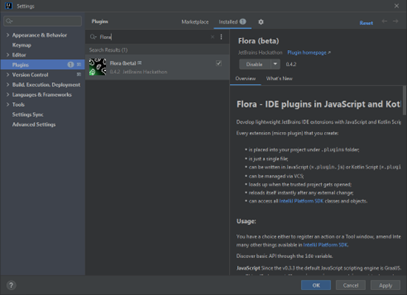
\includegraphics[width=.95\textwidth]{flora_plugin}}
    \caption{Flora Plugin im IntelliJ Plugin Marketplace.}
    \label{fig:FloraPlugin}
\end{figure}    
 
Das Plugin sucht dann in den geöffneten Projektverzeichnissen nach ausführbaren 
„micro plugin“-Dateien, die JavaScript oder Kotlin-Quellcode enthalten. 
Diese müssen sich in einem Ordner namens \emph{.plugins} 
befinden und auf \emph{.plugin.js}  oder \emph{.plugin.kts}  enden \cite{FloraPluginMarketplace}.
Innerhalb dieser Plugin-Dateien kann über die Variable \emph{ide} auf 
die angebotene Schnittstelle zugegriffen werden. Diese erlaubt 
es unter anderem Actions, Keyboard Shortcuts, Services und 
ToolWindows zu erstellen.

\begin{figure}
    \centering
    \fbox{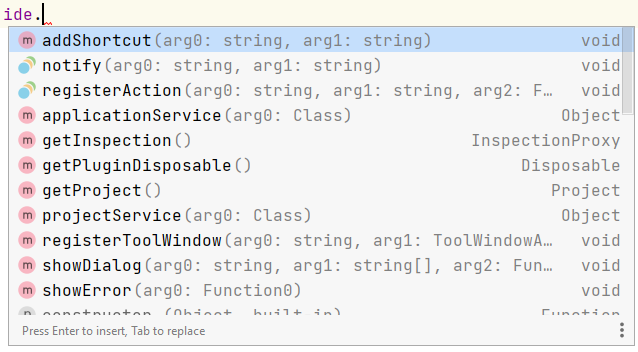
\includegraphics[width=.75\textwidth]{flora_codeCompletion}}
    \caption{Übersicht über die API des Flora Plugins.}
    \label{fig:FloraPluginAPI}
\end{figure}    
 
Flora Plugins bieten sich vor allem dann an, wenn eine projektspezifische 
Aufgabe automatisiert werden soll. Hier sind vor allem die 
Leichtgewichtigkeit der Plugins und die Schnelle, mit der ein 
einfaches Plugin entwickelt werden kann, von großem Vorteil. 
Weiters spricht für diesen Anwendungsfall, dass der Plugin Code 
direkt im Projektordner abgelegt wird und somit auch in einem Version 
Control System wie Git mit abgelegt werden kann.

% //TODO FIX manual \linebreak in multiple places 